\subsection{Введение в метод конечных элементов}

Метод конечных элементов(МКЭ) — это численная процедура решения задач,
сформулированных в виде дифференциального уравнения или вариационного 
принципа.[2]
МКЭ возник как универсальный метод для решения дифференциальных уравнений. 
Метод приобрел большую популярность, так как он позволяет анализировать и
решать широкий спектр задач.


В отличии от других методов, метод конечных элементов имеент одну особенность.
В данном методе аппроксимирующая функция является комбинацией кусочно-гладких конечных функций.
Данные функции являются ненулевыми только в определенном интервале(в методе конечных элементов такие интервалы
называются конечными элементами, на которые, собственно и разбивается область $\Omega$.

Сам метод конечных элементов включает в себя достаточно много технологий. 
Процесс построения решения для данного метода включает
определенную последовательность шагов. Перечислим эти шаги.

1. Для начала необходимо посторить сетку для нашей области $\Omega$.
Для задания коэффициентов уравнений, надо знать определенные свойства материала.
Область $\Omega$ в нашем случае необходима быть покрыта подобластями, удовлетворяющим свойствам - 
они все должны быть попарно непересекаемыми[3]. Такие подобласти и называются конечными элементами (КЭ)(Рисунок 1).

\renewcommand{\figurename}{Рисунок}
\begin{figure}[H]
      \centering
      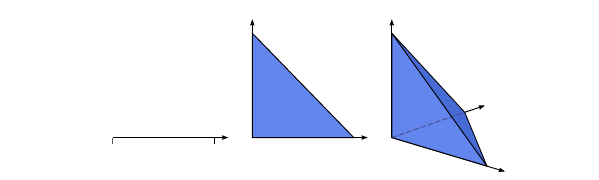
\includegraphics[width=0.8\textwidth]{./pics/random-cells.png}\\
      \centering\caption{Пример конечно-элементных подобластей для пространств размерности n = 1,2,3}
\end{figure}
Соответственно, совокупность всех КЭ называется конечно-элементной сеткой[4].
Вершины конечных элементов называются узлами. Узлы бывают двух типов: внешние и внутренние.
На границах конечных элементов расположены внешние узлы(они соединяют соседние КЭ).
Внутренние узлы конечного элемента используются для более конкретного описания искомых функций[3].

Рассмотрим решение в узле. Части решения в конкретном узле называются степенями свободы.
Понятно, что в зависимости от типа задачи число степеней свободы
в узле различно. В задаче теплопроводности, например, ищется одно значение температуры(одна степень свободы)[3].
В случае двумерной задачи упругости, число частей решения будет равно двум(т.к. $u=(ux, uy)$.
    Значения функции в узлах могут фигурировать в качестве степеней свободы[3].
Важно знать материал, который присутствует в задаче. В нашем случае из этого материала 
сделаны сами конечные элементы.

Как только область разбита на соответствующие подобласти, на каждой такой подобласти можно 
определить функциональное пространство $V$ и использовать каждое $V$ для определения глобального
функционального пространства $V_h$. Подобласть $T$ вместе с определенным на ней функциональным пространством $V$ называется конечным элементом. Более строгое определение:

\begin{itemize}
    \item Подобласть $T$ - замкнута, с кусочно-гладкой границей
    \item Область $V(T)$ - конечное функциональное пространство на $T$
\end{itemize}

2. Приведение поиска решения к решению обычной системы линейных уравнений с учетом граничных условий.

3. Решение полученной системы уравнений.
После решения данной системы, мы получим коэффициенты. Причем, так как на каждом КЭ 
мы задали функциональное пространство и базисные функции, то после отыскания
коэффициентов решения, наше решение не только будет совпадать в узлах сетки: $u_h(x_i, t) = u(x_i, t) = u_i^t$,
а так же являться непрерывным в остальных точках[4].
